%% rnaastex.cls is the classfile used for Research Notes. It is derived
%% from aastex61.cls with a few tweaks to allow for the unique format required.
%% (10/15/17)
%%\documentclass{rnaastex}

%% Better is to use the "RNAAS" style option in AASTeX v6.2
%% (01/08/18)
\documentclass[RNAAS]{aastex62}

%% Define new commands here
\newcommand\latex{La\TeX}

%% Tells LaTeX to search for image files in the 
%% current directory as well as in the figures/ folder.
\graphicspath{{./}{figures/}}

\begin{document}

\title{An example of a Research Note of the American Astronomical Society (RNAAS)}

%% Note that the corresponding author command and emails has to come
%% before everything else. Also place all the emails in the \email
%% command instead of using multiple \email calls.
\correspondingauthor{August Muench}
\email{greg.schwarz@aas.org, august.muench@aas.org}

\author{Ethan Vishniac}
\altaffiliation{Editor-in-Chief}
\affiliation{Johns Hopkins University}

\author{Chris Lintott}
\altaffiliation{RNAAS Editor}
\affiliation{Oxford University}

%% The \author command can take an optional ORCID.
\author[0000-0002-0786-7307]{Greg J. Schwarz}
\affiliation{American Astronomical Society \\
2000 Florida Ave., NW, Suite 300 \\
Washington, DC 20009-1231, USA}

\author{August Muench}
\affiliation{American Astronomical Society \\
2000 Florida Ave., NW, Suite 300 \\
Washington, DC 20009-1231, USA}

%% Note that RNAAS manuscripts DO NOT have abstracts.
%% See the online documentation for the full list of available subject
%% keywords and the rules for their use.
\keywords{editorials, notices --- 
miscellaneous --- catalogs --- surveys}

%% Start the main body of the article. If no sections in the 
%% research note leave the \section call blank to make the title.
\section{} 

\textit{Research Notes of the \href{https://aas.org}{American Astronomical Society}}
(\href{http://rnaas.aas.org}{RNAAS}) is a publication in the AAS portfolio
(alongside ApJ, AJ, ApJ Supplements, and ApJ Letters) through which authors can 
promptly and briefly share materials of interest with the astronomical community
in a form that will be searchable via ADS and permanently archived.

The astronomical community has long faced a challenge in disseminating
information that may not meet the criteria for a traditional journal article.
There have generally been few options available for sharing works in progress,
comments and clarifications, null results, and timely reports of observations
(such as the spectrum of a supernova), as well as results that wouldn’t
traditionally merit a full paper (such as the discovery of a single exoplanet
or contributions to the monitoring of variable sources). 

Launched in 2017, RNAAS was developed as a supported and long-term
communication channel for results such as these that would otherwise be
difficult to broadly disseminate to the professional community and persistently
archive for future reference.

Submissions to RNAAS should be brief communications - 1,000 words or fewer
\footnote{An easy way to count the number of words in a Research Note is to use
the \texttt{texcount} utility installed with most \latex\ installations. The
call  \texttt{texcount -incbib -v3 rnaas.tex}) gives 57 words in the front
matter and 493 words in the text/references/captions of this template. Another
option is by copying the words into MS/Word, and using ``Word Count'' under the
Tool tab.}, and no more than a single figure (e.g. Figure \ref{fig:1}) or table
(but not both) - and should be written in a style similar to that of a
traditional journal article, including references, where appropriate, but not
including an abstract.

Unlike the other journals in the AAS portfolio, RNAAS publications are not
peer reviewed; they are, however, reviewed by an editor for appropriateness
and format before publication. If accepted, RNAAS submissions are typically
published within 72 hours of manuscript receipt. Each RNAAS article is
issued a DOI and indexed by ADS \citep{2000A&AS..143...41K} to create a
long-term, citable record of work.

Articles can be submitted in \latex\ (preferably with the new "RNAAS"
style option in AASTeX v6.2), MS/Word, or via the direct submission in the
\href{http://www.authorea.com}{Authorea} or
\href{http://www.overleaf.com}{Overleaf} online collaborative editors.

Authors are expected to follow the AAS's ethics \citep{2006ApJ...652..847K},
including guidance on plagiarism \citep{2012AAS...21920404V}.

%% An example figure call using \includegraphics
\begin{figure}[h!]
\begin{center}
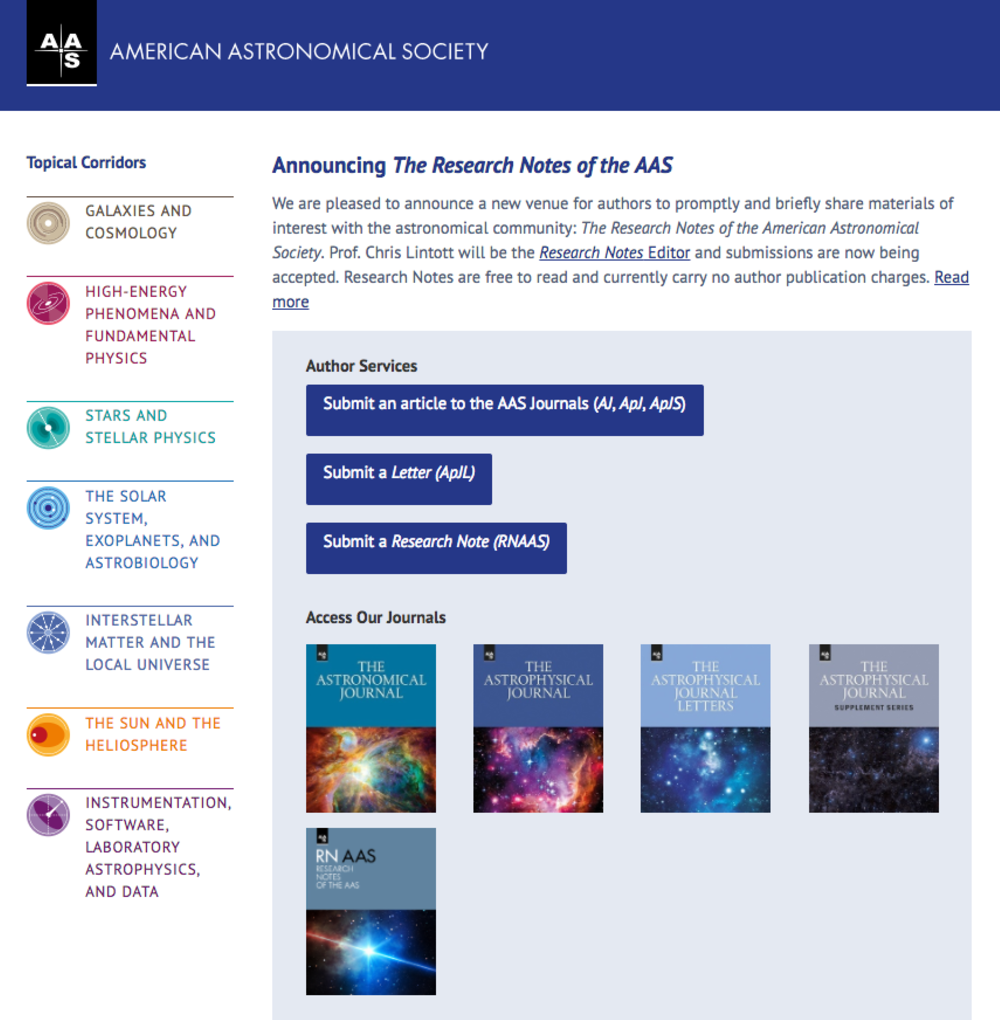
\includegraphics[scale=0.85,angle=0]{aas.pdf}
\caption{Top page of the AAS Journals' website, \url{http://journals.aas.org},
on October 15, 2017.  Each RNAAS manuscript is only allowed one figure or
table (but not both). Including the
\href{http://journals.aas.org//authors/data.html\#DbF}{data behind the figure}
in a Note is encouraged, and the data will be provided as a link in the
published Note.\label{fig:1}}
\end{center}
\end{figure}

%% An example table using AASTeX's deluxetable. Note that since
%% only one figure OR one table is allowed this is commented out.
%\begin{deluxetable}{ccl}
%\tablecaption{Example table some English and Greek letters\label{tab:1}}
%\tablehead{
%\colhead{Index number} & \colhead{English} & \colhead{Greek}
%}
%\startdata
%1 & a & alpha ($\alpha$) \\
%2 & b & beta ($\beta$) \\
%3 & c & gamma ($\gamma$) \\
%4 & d & delta ($\delta$) \\
%5 & e & epsilon ($\epsilon$) \\
%\enddata
%\tablecomments{Long tables should only show a short example with the full
%version as a machine readable table with the article.}
%\end{deluxetable}  

\acknowledgments

Acknowledge people, facilities, and software here but remember that this counts
against your 1000 word limit.

\begin{thebibliography}{}

\bibitem[Kennicutt et al.(2006)]{2006ApJ...652..847K} Kennicutt, R.~C., Jr., Vishniac, E., \& Sneden, C.\ 2006, \apj, 652, 847 

\bibitem[Kurtz et al.(2000)]{2000A&AS..143...41K} Kurtz, M.~J., Eichhorn, G., Accomazzi, A., et al.\ 2000, \aaps, 143, 41 

\bibitem[Vishniac(2012)]{2012AAS...21920404V} Vishniac, E.~T.\ 2012, American Astronomical Society Meeting Abstracts \#219, 219, 204.04 

\end{thebibliography}

\end{document}
